\chapter{Kubernetes}

Kubernetes takes into consideration the following questions:
\begin{itemize}
   \item What happens if a container crashes?
   \item What happens if the machine running a container fails?
   \item How to handle communication between multiple containers how to enable a network between them?
   \item In a multi-machine system, which one should run a container?
\end{itemize}

The answer is \textbf{container orchestration}, implemented by the de facto standard \textit{Kubernetes}:\\
\textbf{K8s} manages the entire \textbf{lifecycle} of individual containers, \textit{spinning up} and \textit{shutting down} resources as needed,
e.g.
if a container shuts down unexpectedly, K8s reacts by launching another container in its place.\\
K8s provides a mechanism for applications to \textbf{communicate} with each other
even as underlying individual containers are created and destroyed.\\
Given a set of container \textbf{\textit{workloads}}\footnote{Rings a bell? Discussed in IRA's course when talking about \textbf{network microsegmentation}} to run and a set of machines on a cluster,
the container orchestrator examines each container and \textbf{determines} the
\textbf{optimal machine} to schedule that workload.

\section{Design Principles}
One of the key points of K8s is the \textit{\textbf{declarativeness}}:
it allows us to simply define the \textbf{desidered state} of our system,
and it will automatically detect and intervene in case the state doesn't meet the specified needs.

Such desired state is defined as a collection of \textbf{objects}:
\begin{itemize}
   \item each object has a specification in which you provide the desired state and a status which reflects the current state of the object
   \item K8s constantly polls each object to ensure that its status is equal to the specification
   \item if an object is unresponsive, K8s will spin up a new version to replace it
   \item if a object's status has drifted from the specification, K8s will issue the necessary commands
   to drive that object back to its desired state
\end{itemize}


K8s integrates perfectly with microservice-based architecture and with the principle of \textit{\textbf{decoupling}},
i.e. decomposing a system into smaller \textit{decoupled} services which can be scaled and updated independently.

K8s is designed in a way which implies that to get the most from containers and container orchestration,
deploying \textit{\textbf{immutable infrastructure}} should be preferred.
\textit{Immutable}, even if it seems odd, indicates that containers shouldn't be too complicate ar alter their state,
and that the user shouldn't, for example, log into a container and change libraries, code etc.
Instead, since containers are by nature \textbf{ephimeral},
once there's an update,
a new container image should be built, instantiated and replace the old one.
This also allows easy roll-back by simply going back to a previous container image.

\section{K8s Objects}
\subsection{Pod}
\textbf{Pod}s consists of one or more (tightly related!) \textit{containers}, a shared \textit{networking layer} and shared \textit{filesystem volumes}.

\subsection{Deployment}
\begin{figure}[htbp]
   \centering
   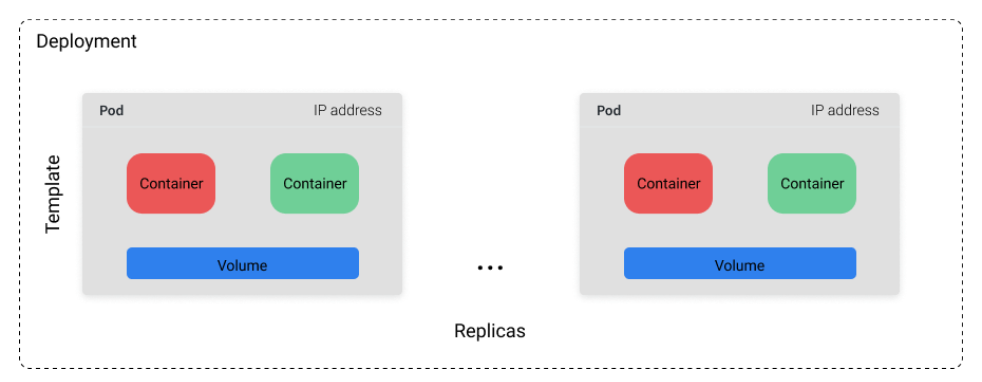
\includegraphics{images/K8s_deployment.png}
   \caption{Deployment Object}
   \label{fig:K8s_deployment}
\end{figure}

A \textbf{Deployment} object includes a collection of Pods defined by a template and a \textit{replica count},
indicating how many copies of the template should be running.

The cluster will always try to have $n$ Pods available
e.g. if we define a deployment with a replica count of 10 and 3 of those Pods crash, 3
more Pods will be scheduled to run on a different machine in the cluster.

\subsection{Service}
\textit{Each Pod} is assigned a \textbf{unique IP} address that we can use to communicate with it;
a legit question may arise:
How to communicate with Pods if the set of Pods running as part of the Deployment can change at any time?

\begin{figure}[htbp]
   \centering
   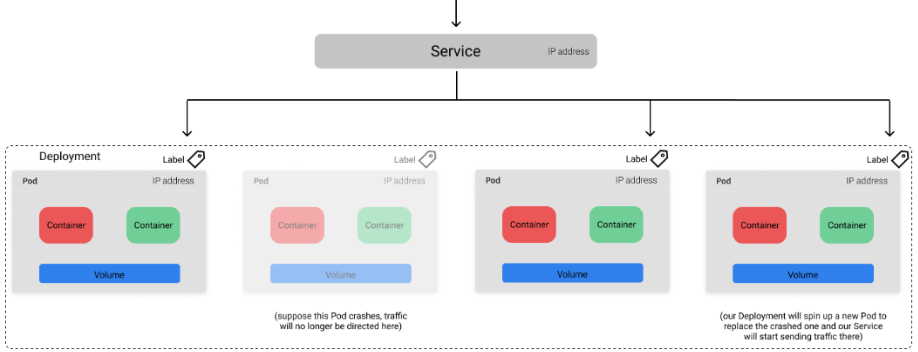
\includegraphics{images/K8s_service.png}
   \caption{Service Object}
   \label{fig:K8s_service}
\end{figure}

K8s \textbf{Service} object provides a stable endpoint to direct traffic to the desired Pods
even as the exact underlying Pods change due to updates/scaling/failures.\\
Services know which Pods they should send traffic to based on labels ($\langle \textit{key-value},\textit{pairs}\rangle$) which we define in the Pod \textit{metadata}.

\subsection{Ingress}
\textit{Service} objects allows us to \textbf{expose} applications behind a stable endpoint only available to internal cluster traffic;\\
To expose our application to traffic \textit{external} to our cluster, we need to
define an \textbf{Ingress} object, which allows to select which Services to make publicly available.

\begin{figure}[htbp]
   \centering
   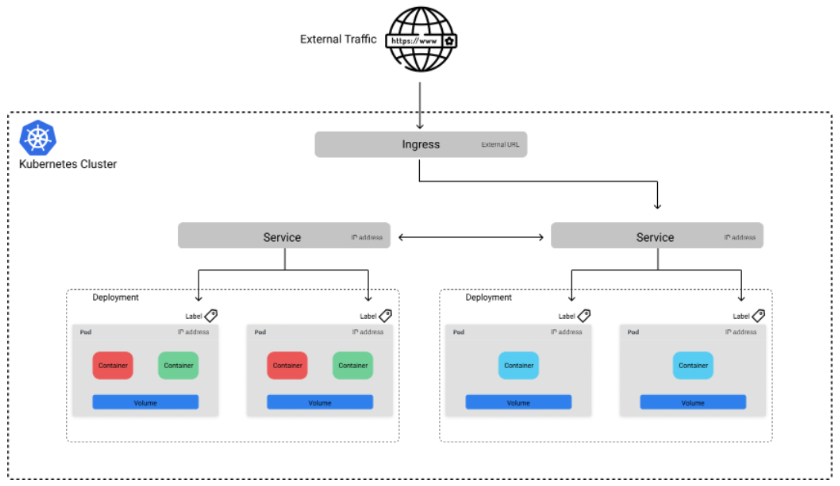
\includegraphics{images/K8s_ingress.png}
   \caption{Ingress Object}
   \label{fig:K8s_ingress}
\end{figure}

\subsection*{Others - Not discussed}

\section{Control Plane}
Two types of machines in a cluster:
\begin{enumerate}
   \item \textbf{master node} - (often single) machine that contains most of the control plane components
   \item \textbf{worker node} - machine that runs the application workloads
\end{enumerate}

Let's dig into the components of both node types.

\subsection{Master node}

User provides new/updated object specification to \textbf{API server} of master node, 
which
validates update requests and acts as unified interface for questions about cluster's \textit{current state},
stored in a distributed key-value store \texttt{etcd}


The \textbf{scheduler} determines where objects should be run
\begin{itemize}
   \item asks the API server which objects haven't been assigned to a machine
   \item determines which machines those objects should be assigned to
   \item replies back to the API server to reflect this assignment
\end{itemize}

The \textbf{controller-manager} monitors cluster state through the API server, 
and in case the actual state differs from desired state,
the controller-manager will make changes via the API server to drive the cluster towards the desired state.

\subsection{Worker node}

The \textbf{kubelet} act a node's "agent" which communicates with
the API server to see which container workloads have been assigned to the node.
It responsible for spinning up pods to run these
assigned workloads, and for announcing {---} when a node first joins the cluster {---} a node's existence to the API server,
so that the scheduler can assign pods to it.

\textbf{kube-proxy} enables containers to communicate with each other across the various nodes on the cluster.

Besides these two components there only \textbf{Pods} left, discussed earlies.

\section{Concluding remarks}
When should you \textbf{\textit{not}} use \textit{K8s}?
\begin{itemize}
   \item If you can run your workload on a single machine
   \item If your compute needs are light
   \item If you don't need high availability and can tolerate downtime
   \item If you don't envision making a lot of changes to your deployed services
   \item If you have a monolith and don't plan to break it into microservices
\end{itemize}

Besides this,
a simpler yet less powerful alternative is \href{https://docs.docker.com/engine/swarm/}{\textit{Docker-swarm}},
usually preferred in environments where simplicity and fast development are prioritized.